\documentclass{standalone}
\usepackage{tikz}
\usetikzlibrary{patterns, positioning}

\begin{document}
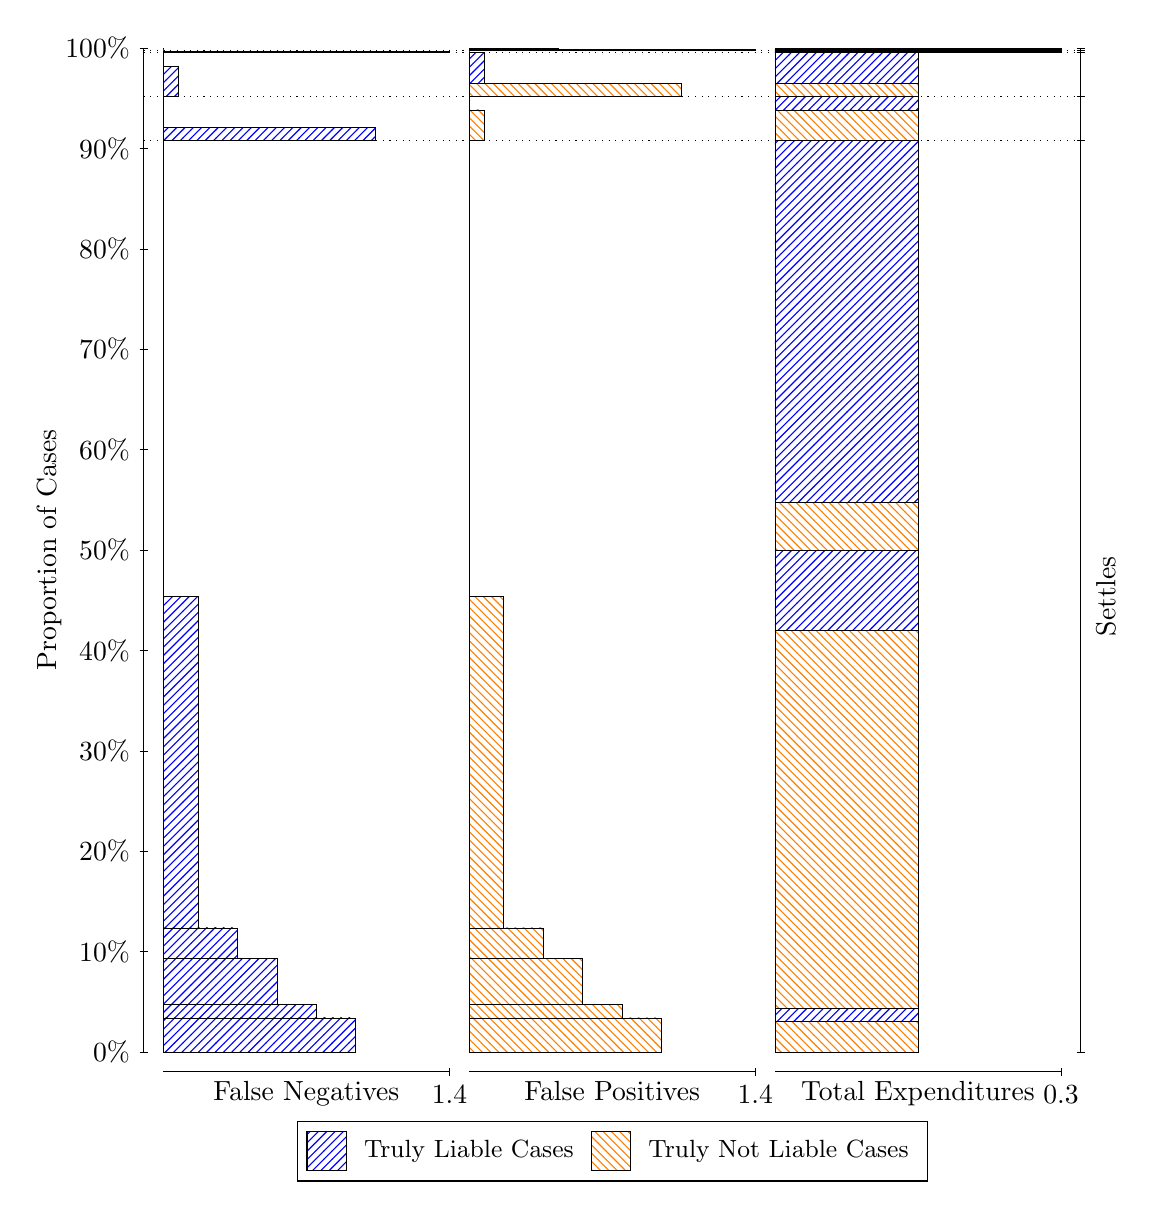
\begin{tikzpicture}
\draw[black, very thin] (1.5,1.75) -- (1.5,14.5);
\node[rotate=90, anchor=center] at (0.3, 8.125) {Proportion of Cases};
\draw[black, very thin] (1.45,1.75) -- (1.55,1.75);
\node[anchor=east] at (1.45, 1.75) {0\%};
\draw[black, very thin] (1.45,3.025) -- (1.55,3.025);
\node[anchor=east] at (1.45, 3.025) {10\%};
\draw[black, very thin] (1.45,4.3) -- (1.55,4.3);
\node[anchor=east] at (1.45, 4.3) {20\%};
\draw[black, very thin] (1.45,5.575) -- (1.55,5.575);
\node[anchor=east] at (1.45, 5.575) {30\%};
\draw[black, very thin] (1.45,6.85) -- (1.55,6.85);
\node[anchor=east] at (1.45, 6.85) {40\%};
\draw[black, very thin] (1.45,8.125) -- (1.55,8.125);
\node[anchor=east] at (1.45, 8.125) {50\%};
\draw[black, very thin] (1.45,9.4) -- (1.55,9.4);
\node[anchor=east] at (1.45, 9.4) {60\%};
\draw[black, very thin] (1.45,10.675) -- (1.55,10.675);
\node[anchor=east] at (1.45, 10.675) {70\%};
\draw[black, very thin] (1.45,11.95) -- (1.55,11.95);
\node[anchor=east] at (1.45, 11.95) {80\%};
\draw[black, very thin] (1.45,13.225) -- (1.55,13.225);
\node[anchor=east] at (1.45, 13.225) {90\%};
\draw[black, very thin] (1.45,14.5) -- (1.55,14.5);
\node[anchor=east] at (1.45, 14.5) {100\%};

\draw[black, very thin] (13.4,1.75) -- (13.4,14.5);
\draw[black, very thin] (13.35,1.75) -- (13.45,1.75);
\node[anchor=west] at (13.35, 1.75) {};
\draw[black, very thin] (13.35,13.326) -- (13.45,13.326);
\node[anchor=west] at (13.35, 13.326) {};
\draw[black, very thin] (13.35,13.883) -- (13.45,13.883);
\node[anchor=west] at (13.35, 13.883) {};
\draw[black, very thin] (13.35,14.441) -- (13.45,14.441);
\node[anchor=west] at (13.35, 14.441) {};
\draw[black, very thin] (13.35,14.47) -- (13.45,14.47);
\node[anchor=west] at (13.35, 14.47) {};
\draw[black, very thin] (13.35,14.5) -- (13.45,14.5);
\node[anchor=west] at (13.35, 14.5) {};

\draw[black, very thin, pattern color=blue, pattern=north east lines] (1.75,1.75) rectangle (4.1931,2.1825);
\draw[black, very thin, pattern color=blue, pattern=north east lines] (1.75,2.1825) rectangle (3.692,2.3531);
\draw[black, very thin, pattern color=blue, pattern=north east lines] (1.75,2.3531) rectangle (3.1908,2.9401);
\draw[black, very thin, pattern color=blue, pattern=north east lines] (1.75,2.9401) rectangle (2.6897,3.3271);
\draw[black, very thin, pattern color=blue, pattern=north east lines] (1.75,3.3271) rectangle (2.1885,7.5379);
\draw[black, very thin, pattern color=orange, pattern=north west lines] (1.75,7.5379) rectangle (1.75,13.326);
\draw[black, very thin, pattern color=blue, pattern=north east lines] (1.75,13.326) rectangle (4.4437,13.496);
\draw[black, very thin, pattern color=orange, pattern=north west lines] (1.75,13.496) rectangle (1.75,13.883);
\draw[black, very thin, pattern color=blue, pattern=north east lines] (1.75,13.883) rectangle (1.9379,14.27);
\draw[black, very thin, pattern color=orange, pattern=north west lines] (1.75,14.27) rectangle (1.75,14.441);
\draw[black, very thin, pattern color=blue, pattern=north east lines] (1.75,14.441) rectangle (5.3833,14.455);
\draw[black, very thin, pattern color=orange, pattern=north west lines] (1.75,14.455) rectangle (1.75,14.47);
\draw[black, very thin, pattern color=orange, pattern=north west lines] (1.75,14.47) rectangle (1.75,14.484);
\draw[black, very thin, pattern color=blue, pattern=north east lines] (1.75,14.484) rectangle (1.75,14.5);
\draw[black, very thin, pattern color=orange, pattern=north west lines] (5.6333,1.75) rectangle (8.0764,2.1825);
\draw[black, very thin, pattern color=orange, pattern=north west lines] (5.6333,2.1825) rectangle (7.5753,2.3532);
\draw[black, very thin, pattern color=orange, pattern=north west lines] (5.6333,2.3532) rectangle (7.0741,2.9401);
\draw[black, very thin, pattern color=orange, pattern=north west lines] (5.6333,2.9401) rectangle (6.573,3.3271);
\draw[black, very thin, pattern color=orange, pattern=north west lines] (5.6333,3.3271) rectangle (6.0718,7.5378);
\draw[black, very thin, pattern color=blue, pattern=north east lines] (5.6333,7.5378) rectangle (5.6333,13.326);
\draw[black, very thin, pattern color=orange, pattern=north west lines] (5.6333,13.326) rectangle (5.8213,13.713);
\draw[black, very thin, pattern color=blue, pattern=north east lines] (5.6333,13.713) rectangle (5.6333,13.883);
\draw[black, very thin, pattern color=orange, pattern=north west lines] (5.6333,13.883) rectangle (8.327,14.054);
\draw[black, very thin, pattern color=blue, pattern=north east lines] (5.6333,14.054) rectangle (5.8213,14.441);
\draw[black, very thin, pattern color=orange, pattern=north west lines] (5.6333,14.441) rectangle (5.6333,14.456);
\draw[black, very thin, pattern color=blue, pattern=north east lines] (5.6333,14.456) rectangle (5.6333,14.47);
\draw[black, very thin, pattern color=orange, pattern=north west lines] (5.6333,14.47) rectangle (9.2667,14.484);
\draw[black, very thin, pattern color=blue, pattern=north east lines] (5.6333,14.484) rectangle (6.7609,14.5);
\draw[black, very thin, pattern color=orange, pattern=north west lines] (9.5167,1.75) rectangle (11.333,2.1369);
\draw[black, very thin, pattern color=blue, pattern=north east lines] (9.5167,2.1369) rectangle (11.333,2.3075);
\draw[black, very thin, pattern color=orange, pattern=north west lines] (9.5167,2.3075) rectangle (11.333,7.1052);
\draw[black, very thin, pattern color=blue, pattern=north east lines] (9.5167,7.1052) rectangle (11.333,8.1247);
\draw[black, very thin, pattern color=orange, pattern=north west lines] (9.5167,8.1247) rectangle (11.333,8.7279);
\draw[black, very thin, pattern color=blue, pattern=north east lines] (9.5167,8.7279) rectangle (11.333,13.326);
\draw[black, very thin, pattern color=orange, pattern=north west lines] (9.5167,13.326) rectangle (11.333,13.713);
\draw[black, very thin, pattern color=blue, pattern=north east lines] (9.5167,13.713) rectangle (11.333,13.883);
\draw[black, very thin, pattern color=orange, pattern=north west lines] (9.5167,13.883) rectangle (11.333,14.054);
\draw[black, very thin, pattern color=blue, pattern=north east lines] (9.5167,14.054) rectangle (11.333,14.441);
\draw[black, very thin, pattern color=orange, pattern=north west lines] (9.5167,14.441) rectangle (13.15,14.456);
\draw[black, very thin, pattern color=blue, pattern=north east lines] (9.5167,14.456) rectangle (13.15,14.47);
\draw[black, very thin, pattern color=orange, pattern=north west lines] (9.5167,14.47) rectangle (13.15,14.484);
\draw[black, very thin, pattern color=blue, pattern=north east lines] (9.5167,14.484) rectangle (13.15,14.5);
\draw[black, dotted] (1.5,13.326) -- (13.4,13.326);
\draw[black, dotted] (1.5,13.883) -- (13.4,13.883);
\draw[black, dotted] (1.5,14.441) -- (13.4,14.441);
\draw[black, dotted] (1.5,14.47) -- (13.4,14.47);
\draw[black, very thin] (1.75,1.5) -- (5.3833,1.5);
\node[anchor=north] at (3.5667, 1.5) {False Negatives};
\draw[black, very thin] (5.3833,1.45) -- (5.3833,1.55);
\node[anchor=north] at (5.3833, 1.45) {1.4};

\draw[black, very thin] (5.6333,1.5) -- (9.2667,1.5);
\node[anchor=north] at (7.45, 1.5) {False Positives};
\draw[black, very thin] (9.2667,1.45) -- (9.2667,1.55);
\node[anchor=north] at (9.2667, 1.45) {1.4};

\draw[black, very thin] (9.5167,1.5) -- (13.15,1.5);
\node[anchor=north] at (11.333, 1.5) {Total Expenditures};
\draw[black, very thin] (13.15,1.45) -- (13.15,1.55);
\node[anchor=north] at (13.15, 1.45) {0.3};

\node[black, centered, rotate=90] at (13.72, 7.5378) {Settles};





\draw (7.449999999999999,1.5) node[draw=none] (baseCoordinate) {};
\begin{scope}[align=center]
        \matrix[scale=0.5, draw=black, below=0.5cm of baseCoordinate, nodes={draw}, column sep=0.1cm]{
            \node[rectangle, draw, minimum width=0.5cm, minimum height=0.5cm, pattern=north east lines, pattern color=blue] {}; &
            \node[draw=none, font=\small] (B) {Truly Liable Cases}; &
            \node[rectangle, draw, minimum width=0.5cm, minimum height=0.5cm, pattern=north west lines, pattern color=orange] {}; &
            \node[draw=none, font=\small] (B) {Truly Not Liable Cases}; \\
            };
\end{scope}

\end{tikzpicture}
\end{document}